\documentclass[conference]{IEEEtran}
\IEEEoverridecommandlockouts
% The preceding line is only needed to identify funding in the first footnote. If that is unneeded, please comment it out.
\usepackage{cite}
\usepackage{amsmath,amssymb,amsfonts}
\usepackage{algorithmic}
\usepackage{graphicx}
\usepackage{textcomp}
\usepackage{xcolor}
\def\BibTeX{{\rm B\kern-.05em{\sc i\kern-.025em b}\kern-.08em
    T\kern-.1667em\lower.7ex\hbox{E}\kern-.125emX}}
\begin{document}

\title{Predicting the Average Two-Year Win Probability and Hire Tenure of NFL Head Coach Hires: Three Approaches}

\author{\IEEEauthorblockN{Jon C. Williamson}
\IEEEauthorblockA{\textit{Dept. of Computer Science \& Engineering} \\
\textit{Texas A\&M University}\\
College Station, TX, USA \\
jonwilliamson@tamu.edu}
}

\maketitle

\begin{abstract}
This document is a model and instructions for \LaTeX.
This and the IEEEtran.cls file define the components of your paper [title, text, heads, etc.]. *CRITICAL: Do Not Use Symbols, Special Characters, Footnotes, 
or Math in Paper Title or Abstract.
\end{abstract}

\begin{IEEEkeywords}
machine learning, neural networks, prediction methods, supervised learning, unsupervised learning
\end{IEEEkeywords}

\section{Introduction}
Although the National Football League (NFL) is not publicly traded, evaluation of its teams suggests that it is worth over \$91 billion dollars \cite{b1}.  Equivalently, the average NFL franchise is worth \$2.86 billion dollars \cite{b1}. Despite these large evaluations, hiring successful head coaches is anything but repeatable in the NFL. In 2016, the median head coach tenure in position was three years \cite{b2}. Although this length is marginally better than other sports leagues \cite{b2}, comparing the average top job tenure to public sector best practice shows immense area for improvement. A publicly traded company that changed CEOs at this rate would have an extremely volatile stock price and likely decreased stock demand \cite{b3}. In this analogy, the general manager is the entire Board of Directors. Moreover, successful head coach hiring is tremendously valuable, as a differentiated NFL head coach can bring about lasting success and divisional dominance, subsequently increasing the historical importance of a franchise and improving its bottom line. A machine learning model that can increase the hit probability of head coaching hires has the potential to add immense value to NFL franchises. This project attempts to predict two outcomes of head coach hires: the average two-year winning percent and the hire tenure, using three machine learning approaches.

\section{Literature Review}
There have been no journal publications that attempt to predict the success of NFL coaching hires through statistical learning techniques. Currently, the NFL is only beginning to implement artificial intelligence (AI) in play calling prediction \cite{b4}. Additionally, there are few papers that examine the impact of individual features on NFL head coaching success. Reference \cite{b5} used a linear regression with seven features to attempt to predict the number of wins of head coaches in their first three years in order to understand if prior NFL head coaching experience impacts success in position. This paper found that a previous head coaching experience had a negative impact on the success of new head coaches. Despite this finding, the model supported an adjusted $R^2$ of only $0.336$. This low value does not instill confidence in its findings or feature weights. Additionally, the lack of regularization and the small number of features further decrease confidence in the findings. Reference \cite{b6} reviews research in sports economics and suggests that hiring decisions made solely on playing success are unlikely to be optimal given financial (resource) inequality among sports franchises. 

\section{Problem Formulation}
This project develops three implementations of two machine learning models. The first model attempts to predict a coach's average winning probability in their first two years following hiring using three separate regressors. The second model attempts to predict a classification of coach tenure following hiring using three multi-class classifiers. Although the feature set and data points for these problems are largely identical, this report will analyze both models separately.

\section{Proposed Solution}

\subsection{Predicting Average Two-Year Winning Probability}
Equation \eqref{eq1} defines the calculation of average winning probability, $p_{win}$, as a function of the number of wins, $n_{wins}$, the number of losses, $n_{losses}$, and the number of ties, $n_{ties}$, of a head coach over any interval. 

\begin{equation}
        p_{win}=\frac{n_{wins} + 0.5*n_{ties}}{n_{wins} + n_{losses} + n_{ties}}
        \label{eq1}
\end{equation}

This winning probability is bound within $[0, 1]$. Predicting this continuous value requires regression. This project implements three regressors to attempt this prediction: 
\begin{enumerate}
  \item Linear Regression with Lasso Regularization\cite{b7}
  \item XGBoost Regressor\cite{b8}
  \item Multi-layer Perceptron Regressor\cite{b7}
\end{enumerate}

The first implementation of this model is a simple linear model with $\ell_1$ norm regularization. This project uses $\ell_1$ regularization due to its tendency to remove features from the model. The second implementation of the model is an XGBoost Regressor. This regressor uses gradient boosting to build a single predication model through the aggregation of weak learners. This project uses trees as the universal model for the weak learners. The third and final implementation of this model is through a Multi-layer Perceptron Regressor. This regressor is a basic neural network with a final regression node. It extracts features without supervision. This project utilizes extensive cross-validation to determine the optimal values for hyperparameters for each model implementation. 

This project uses root mean squared error (RMSE) as the evaluation metric for these regression models. This metric was chosen for two reasons. Firstly, its dimensions are identical to the dimensions of the prediction variable. Secondly, it punishes outliers greater than absolute error. It is important to note that the thresholds that constitute `good' and `bad' RMSE are impacted by the scale of the prediction. As a result, this project compares model RMSE against the RMSE for predicting the expected outcome in order to understand model performance. 


\subsection{Predicting Coach Tenure Class}
This project defines the tenure of a coach hire as the number of years the hired coach remains in the same position before being fired, leaving, or retiring. A model that predicts this tenure directly would require regression. This level of granularity is not necessary, as there is no meaningful difference between a coach that is in position for ten years and one that is in position for twelve years. As a result, this project maps coach tenures to four tenure classifications in order to convert this problem to a classification. Equation \eqref{eq2} shows the mapping between the coach tenure, $t$, and coach tenure classification label, $C(t)$.
\begin{equation}
        C(t)=
        \begin{cases}
            0 &t \leq 2 		\\
            1 &2 < t \leq 4 \\
            2 &4 < t \leq 7 \\
            3 &t > 7
        \end{cases}
        \label{eq2}
\end{equation}

Equation \eqref{eq2} shows four independent coach tenure classification labels. The shortest tenure class, of one and two years, is intended to capture the worst head coach hires. The next class, of three and four years, is intended to capture coaches that are mediocre, i.e., coaches that teams would be happy to move on from but are not obligated to do so. The third coach tenure class is intended to capture successful head coaches with tenure between five and seven years. The fourth and final class is intended to capture the best coach hires in the history of the NFL, e.g., the Bill Belichick's and Don Shula's of the league.

This model seeks to predict the coaching tenure classification of head coach hires based on statistics available at the time of hiring. This project utilizes three implementations of this model:
\begin{enumerate}
  \item Logistic Regression with Lasso Regularization\cite{b7}
  \item XGBoost\cite{b8}
  \item Multi-layer Perceptron Classifier\cite{b7}
\end{enumerate}
These implementations are analogous to the three models in the previous subsection. The primary difference is that these implementations are classification models and not regression models. As with the previous model, this project utilizes extensive cross-validation to determine hyperparameter values for each implementation. This project uses weighted one-versus-rest (OVR) area under the receiver operating characteristic curve (AUROC) to measure model performance. This performance metric accounts for class imbalance by weighing the OVR AUROC scores for each class by their prevalence in the entire data set.

\section{Data Description}
This project utilizes 25 features, two description labels, and the two model outputs for each head coaching hire. The two descriptive labels are the coach name and the hire year. These labels exist only to better understand the results, and are not included in the prediction method any model. Table \ref{tab1} shows the 25 features used in each model. Abbreviations included in feature descriptions include offensive coordinator (OC), defensive coordinator (DC), and head coach (HC).

\begin{table}[htbp]
\caption{Model Feature List}
\begin{center}
\begin{tabular}{|c||l|}
\hline
\textbf{No.} & \textbf{Description} \\
\hline
\hline
1 & Age at hiring \\
\hline
2 & Number of times previously hired as head coach \\
\hline
3 & Number of years’ experience as college position coach \\
\hline
4 & Number of years’ experience as college coordinator \\
\hline
5 & Number of years’ experience as college head coach \\
\hline
6 & Number of years’ experience as NFL position coach \\
\hline
7 & Number of years’ experience as NFL coordinator \\
\hline
8 & Number of years’ experience as NFL head coach \\
\hline
9 & Demotion presence in hiring history \\
\hline
10 & During years as NFL OC, team’s avg. norm. yardage rank \\
\hline
11 & During years as NFL OC, team’s avg. norm. point rank \\
\hline
12 & During years as NFL OC, team’s avg. norm. giveaway rank \\
\hline
13 & During years as NFL DC, team’s avg. norm. yardage rank \\
\hline
14 & During years as NFL DC, team’s avg. norm. point rank \\
\hline
15 & During years as NFL DC, team’s avg. norm. turnover rank \\
\hline
16 & During years as NFL HC, team’s avg. norm. yardage differential\\
&rank \\
\hline
17 & During years as NFL HC, team’s avg. norm. point differential \\
&rank \\
\hline
18 & During years as NFL HC, team’s avg. norm. turnover ratio rank \\
\hline
19 & Hiring team’s avg. winning percent in previous two years \\
\hline
20 & Hiring team’s avg. norm. turnover ratio rank in previous two \\
&years \\
\hline
21 & Hiring team’s avg. norm. point differential rank in previous\\
& two years \\
\hline
22 & Hiring team’s avg. norm. yard differential rank in previous\\
&two years \\
\hline
23 & Hiring team’s avg. norm. divisional placement in previous two\\
&years \\
\hline
24 & Hiring team’s number of playoff appearances in previous\\
&two years \\
\hline
25 & Hiring team’s number of playoff wins in previous two years \\
\hline
\end{tabular}
\label{tab1}
\end{center}
\end{table}

Table \ref{tab1} shows that features 1 through 18 are characteristics of head coaches at time of hiring, while features 19 through 25 are characteristics of the hiring team. This distinction is essential, as resource inequality among franchises does impact team success independent of any coaching effort \cite{b6}. Moreover, this project includes these team-specific features because the models could determine profiles of successful coaches with respect to team state in order to maximize win total and coach tenure. All features are purely numeric. Only one feature, feature 9, is categorical. All other features are continuous.

Features 10 through 18 and 20 through 23 reference average normalized team ranks in different categories. For these features, the single feature value is taken as the average of the normalized ranks for all years that qualify. A single feature instance prior to averaging for these features is the forms was of $x \text{ out of }z$, where $x$ is the rank of the attribute by team out of $z$ total teams. Equation \eqref{eq3} linearly distributes the feature instance value from $1$ at the best rank to $0$ at the worst rank:

\begin{equation}
        f(x,z) = \frac{z-x}{z-1}
        \label{eq3}
\end{equation}

Raw data was collected by scraping pro-football-reference.com. The crawling script extracted three performance tables for all head coaches in NFL history. For any coach, these three tables detail the top-level coaching results, the team's ranks in many categories relative to the league, and the coach's career hiring record for every year in their career. 

The crawling script also extracted two performance tables for all franchises in NFL history. For any franchise, these two tables include the team's record \& ranks and playoff statistics for every season in franchise history.

A script was written to analyze the crawled data to extract the feature set and calculate the two model outputs for all coach hires in NFL history. It should be noted that this script considers interim promotions acts of coach hiring, as exceptional performance as an interim coach can lead to a non-interim promotion. This script identified 693 hiring instances in the history of the NFL.

Fig. \ref{fig1} shows the corrlation matrix among all 25 features. This matrix shows that the data is not highly correlated. The three-by-three white boxes in the matrix show that there is no correlation among features 10 through 12 and 13 through 15. Features 10 through 12 are based on team performance as an offensive coordinator, while features 13 through 15 are from performance as a defensive coordinator. No coaches in the set were both an OC and a DC prior to being hired, hence there is no correlation value among those features. 

\begin{figure}[htbp]
\centerline{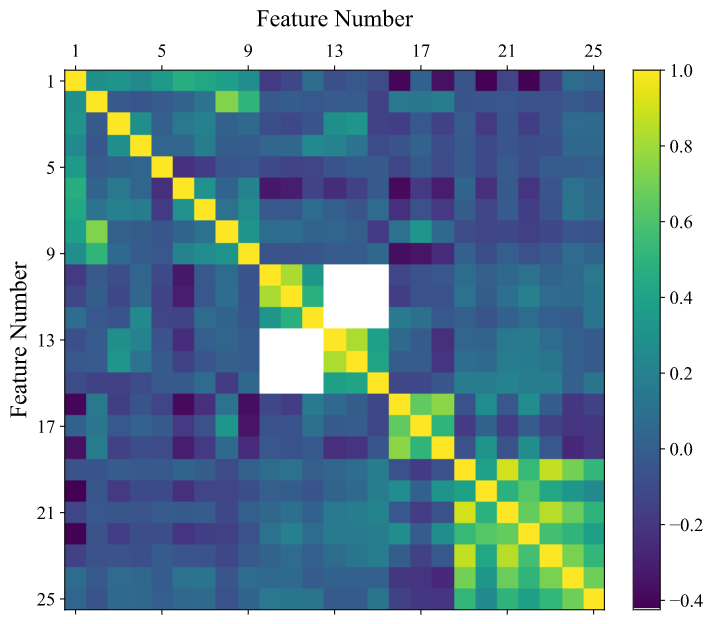
\includegraphics[width=1\linewidth]{corr.png}}
\caption{Feature correlation matrix.}
\label{fig1}
\end{figure}

There is some correlation among features 19 through 25. Recall that these features are characteristics of hiring teams in the two years prior to the coaching hire. It makes some sense that these features are correlated, as teams that perform well in these ranking metrics are likely better teams, and thus, should perform well in other ranking metrics. Lastly, there is correlation between feature 1, age at hiring, with features 2-9, which measure number of years of coaching experience at varying levels. This observed correlation is expected. 

Fig. \ref{fig2} shows a histogram of the two-year average winning probability for the data set. This figure shows that the mean average two-year winning percent for new head coach hires is $0.408$. The data is somewhat normally distributed. It should be noted that the outlying win probabilities are most often a result of interim head coach hires that were not promoted following the completion of the season. These coaches have a smaller sample size for win probability calculation, and thus can achieve extreme win probabilities that are more rare over the course of two complete seasons. 

\begin{figure}[htbp]
\centerline{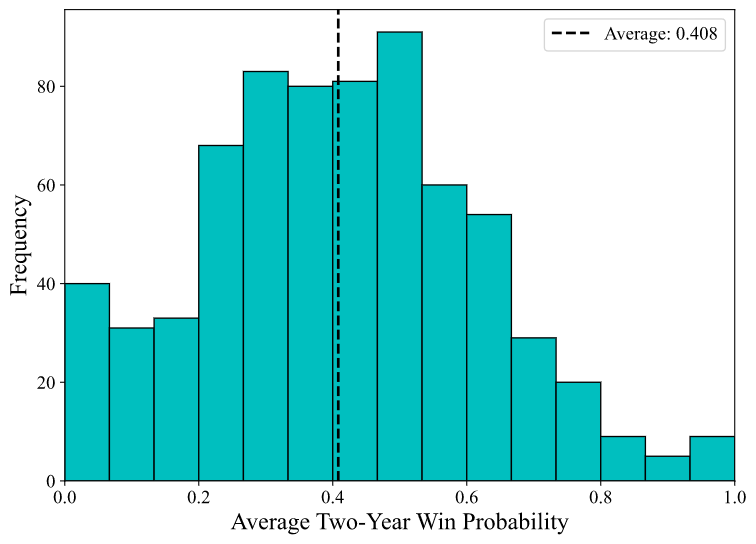
\includegraphics[width=1\linewidth]{hist1.png}}
\caption{Average two-year win probability distribution.}
\label{fig2}
\end{figure}

\begin{figure}[htbp]
\centerline{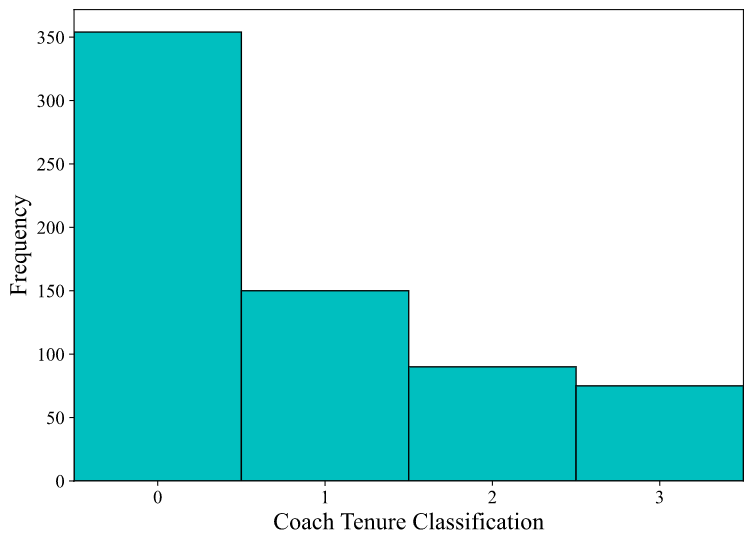
\includegraphics[width=1\linewidth]{hist2.png}}
\caption{Coach tenure classification distribution.}
\label{fig3}
\end{figure}

Fig. \ref{fig3} shows a histogram of coach tenure classification for all head coach hires in the history of the NFL. This figure shows that the data is imbalanced, with frequency of class decreasing with increasing coach tenure. it should be noted that this histogram does not include any currently active head coaches hired during or since 2014, as there has not been enough time for these coaches to be correctly and definitively labeled.

\section{Results}
For all models and all implementations, the data was split into training and validation sets via an 80/20 ratio. Each model was created using multiple levels of internal cross-validation in order to tune hyperparameters. This section reports average RMSE on the training set, the testing set, and the validation set. The testing set is the set of data set aside within internal cross-validation during hyperparameter tuning. The validation set is the 20\% of the entire set that was not used in any portion of training. Do not confuse the testing set and the validation set. Final claims of model performance are made on performance with the validation set.

\subsection{Predicting Average Two-Year Winning Probability}

\subsubsection{Linear Regression with Lasso Regularization}
This implementation used an outer ten-fold cross-validation over an inner five-fold cross-validation, each iterating over $1,000$ values of the regularization parameter alpha \verb|alpha|, to determine the hyperparameter value with the greatest model performance. Following this cross-validation, a single model was built on the entirety of the training set and used to test the validation set. Table \ref{tab2} shows the results of this implementation.



\begin{table}[htbp]
\caption{Regularized Linear Regression RMSE Results}
\begin{center}
\begin{tabular}{|c||c|}
\hline
\textbf{Data Set} & \textbf{RMSE} \\
\hline
\hline
Train & 0.197 \\
\hline
Test & 0.204 \\
\hline
Validation & 0.202 \\
\hline
Validation, Expected Outcome$^{\mathrm{1}}$ & 0.208 \\
\hline
\multicolumn{2}{l}{$^{\mathrm{1}}$Not influenced by the model.}
\end{tabular}
\label{tab2}
\end{center}
\end{table}

\begin{figure}[htbp]
\centerline{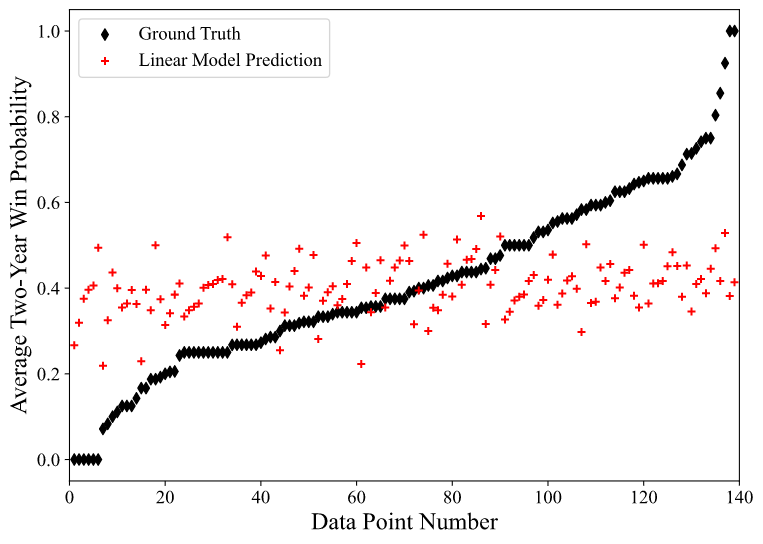
\includegraphics[width=1\linewidth]{test1.png}}
\caption{Validation set, regularized linear model prediction versus ground truth.}
\label{fig4}
\end{figure}

These results show that the regularized linear regression performed marginally better on the validation set than predicting the expected value for the validation set. Fig. \ref{fig4} shows the sorted validation set with corresponding marks for the ground truth values and the predicted values. Fig. \ref{fig4} shows that the regularized linear model tends to predict winning probabilities near the expected value. Additionally, the model's variation in predicted probability is far less than the variation in the testing set. 

\begin{figure}[htbp]
\centerline{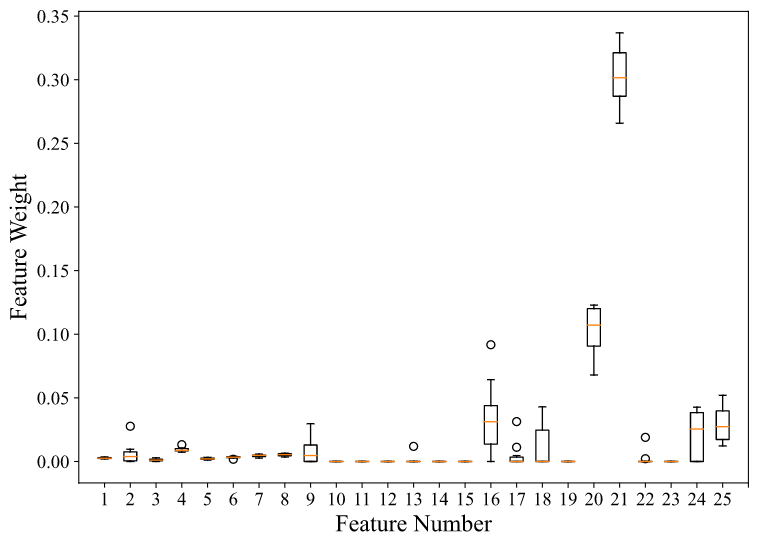
\includegraphics[width=1\linewidth]{weight1.png}}
\caption{Regularized linear model feature weights.}
\label{fig5}
\end{figure}

\subsubsection{XGBoost Regressor}


\subsubsection{Multi-layer Perceptron Regressor}


\subsection{Predicting Coach Tenure Class}
Text

\section{Limitations and Future Directions}

\section{Conclusions}

\begin{thebibliography}{00}
\bibitem{b1} T. Barrabi, ``What is the NFL worth? Revenue, team values and other financial facts,'' Fox Business. https://www.foxbusiness.com/sports/nfl-worthrevenue-team-values (accessed Oct. 26, 2020)
\bibitem{b2} C. Gaines, ``NFL head coaches have good job security when compared to other major sports leagues,'' Business Insider. https://www.businessinsider.com/coaches-managers-tenure-nfl-mlb-nba-nhl-premier-league-2016-12 (accessed Oct. 26, 2020)
\bibitem{b3} ``How does a change in CEO impact stock price?,'' Investopedia. https://www.investopedia.com/ask/answers/010815/how-does-change-ceo-impact-stock-price.asp (accessed Nov. 18, 2020)
\bibitem{b4} ``Using machine learning to peek inside the minds of NFL coaches,'' DataRobot. https://www.datarobot.com/blog/using-machine-learning-to-peek-inside-the-minds-of-nfl-coaches/ (accessed Oct. 26, 2020)
\bibitem{b5} M. Roach, ``Does prior NFL head coaching experience improve team performance?,'' in Journal of Sport Management, vol. 30, no. 3, pp. 298-311.
\bibitem{b6} D. Mielke, ``Coaching experience, playing experience, and coaching tenure: a commentary,'' in International Journal of Sports Science \& Coaching, vol. 2, no. 2, pp. 117-118.
\bibitem{b7} Pedregosa et al., ``Scikit-learn: machine learning in Python,'' in Journal of Machine Learning Research, vol. 12, pp.2825-2830.
\bibitem{b8} T. Chen, and C. Guestrin, ``XGBoost: a scalable tree boosting system,'' in KDD '16: Proceedings of the 22nd ACM SIGKDD International Conference on Knowledge Discovery and Data Mining, pp.785-794.
\end{thebibliography}

\end{document}
